\chapter{Marc Pràctic}
\section{Introducció}\label{sec:intr}
En iniciar la part pràctica del treball vam decidir crear tres tipus de xarxes neuronals: una \nameref{sec:10}, una altra \nameref{sec:11} i, finalment, una \nameref{sec:12}.\\

En aquest capítol explicarem com vam elaborar cadascuna d’aquestes xarxes neuronals i, a més, compararem les dues formes de desenvolupament en una \nameref{sec:op}.\\

Per facilitar l’organització del treball, ens hem repartit les tasques: un membre de l’equip s’ha encarregat de la xarxa neuronal implementada amb llenguatge de programació Python, mentre que l’altre ha treballat una xarxa neuronal feta amb fulls de càlcul. Finalment, hem elaborat conjuntament la taula de comparació, intercanviant perspectives, i també hem treballat plegats la xarxa neuronal del cas real.\\

Les nostres pràctiques consisteixen en recopilar una sèrie de dades d'alumnes mitjançant una enquesta feta per nosaltres amb la finalitat de crear una Xarxa neuronal que pugues predir la nota final de cada alumne. Les preguntes fetes en el formulari són sobre la matèria de matemàtiques i són les següents:
\begin{itemize}
 \item Realització de deures
 \item Hores d'estudis (semanal)
 \item Hores de section
 \item Interès en la matèria
 \item Nota del segon trimestre
 \item Nota del tercer trimestre
 \item Nota final
\end{itemize}
Com es pot veure, les preguntes d'aquest formulari estan relacionades amb el rendiment d'estudis dels alumnes, i s'envia als estudiants que tingues l'assignatura matematiques.
Després de les prediccions, compararem la xarxa neuronal feta amb python y la del full de càlcul i veurem quina de les dos té més precisió.
\begin{comment}
Mostra del formulari:
\begin{figure}[H]
    \centering
    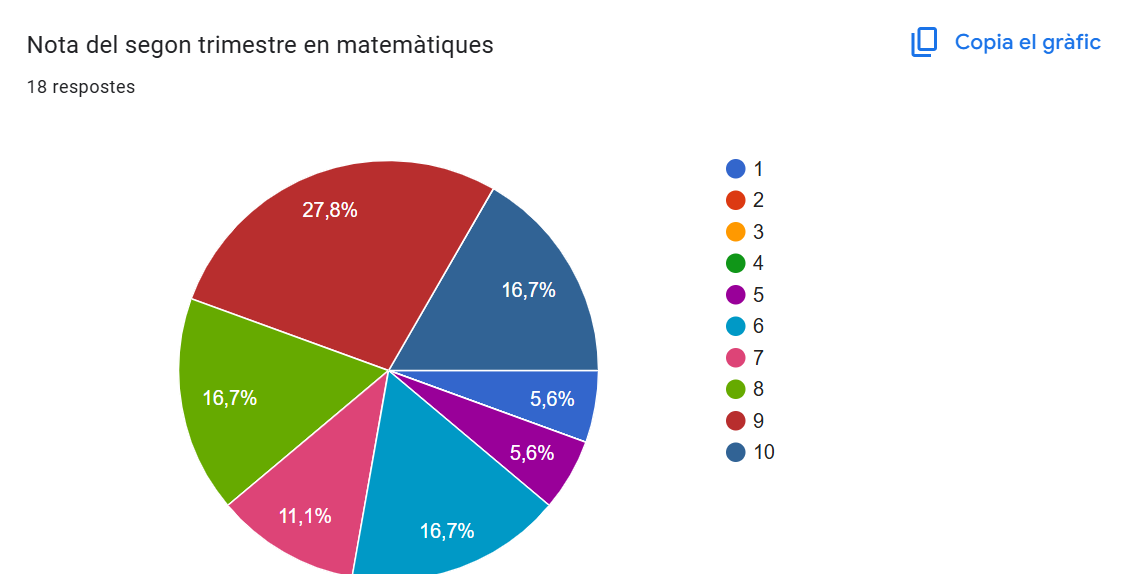
\includegraphics[width=0.5\textwidth]{./figures/14.png}
    \caption{Nota del segon trimestre}
\end{figure}

\begin{figure}[H]
    \centering
    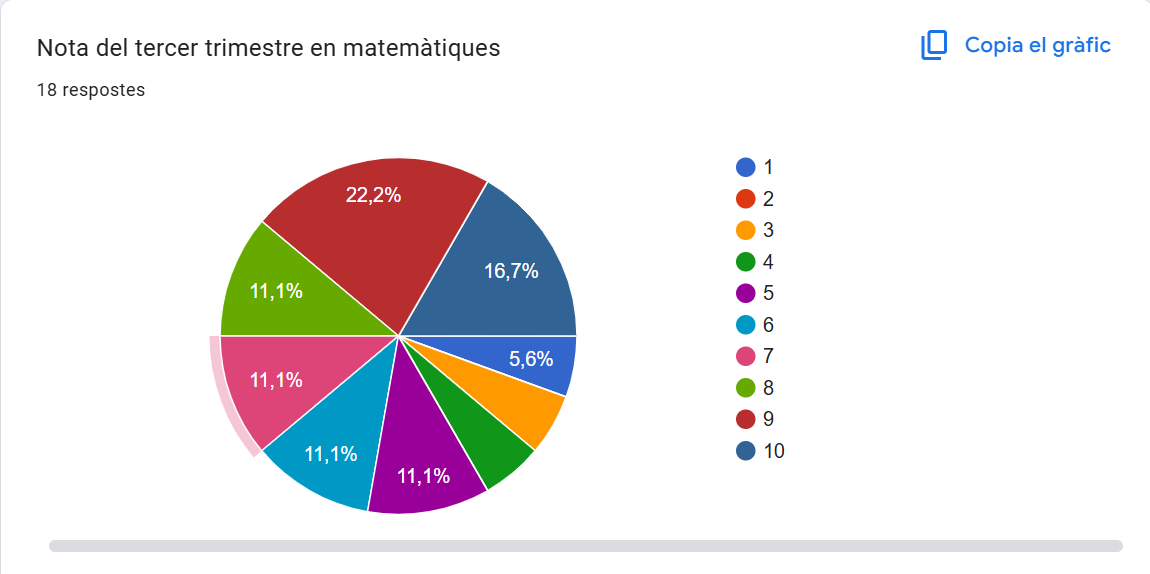
\includegraphics[width=0.5\textwidth]{./figures/15.png}
    \caption{Nota del tercer trimestre}
\end{figure}

\begin{figure}[H]
    \centering
    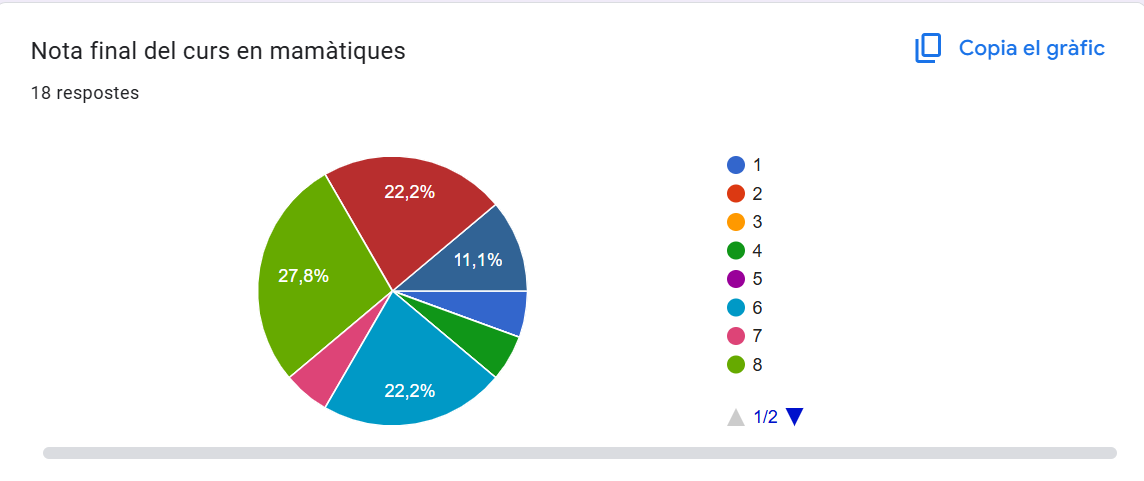
\includegraphics[width=0.5\textwidth]{./figures/16.png}
    \caption{Nota final del curs}
\end{figure}

\begin{figure}[H]
    \centering
    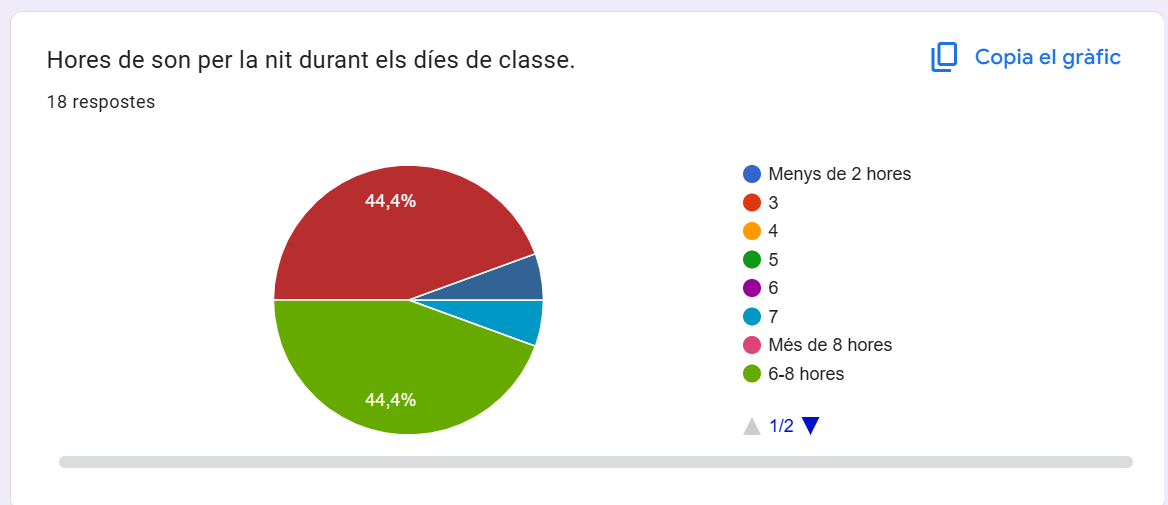
\includegraphics[width=0.5\textwidth]{./figures/17.png}
    \caption{Hores de son per la nit durant l'horari escolar}
\end{figure}

\begin{figure}[H]
    \centering
    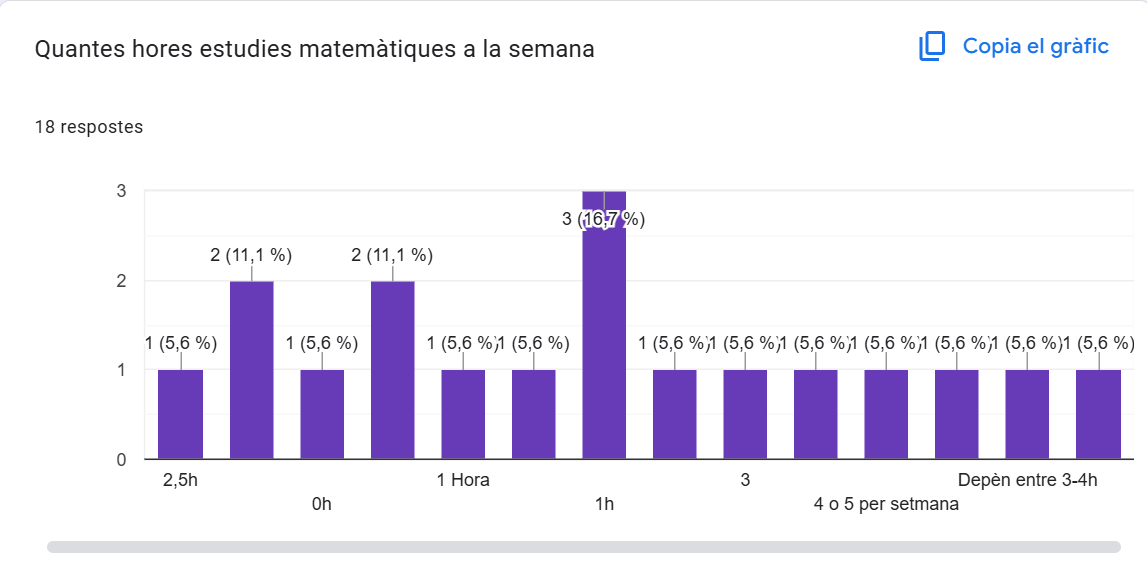
\includegraphics[width=0.5\textwidth]{./figures/18.png}
    \caption{Cuantes hores estudies a la semana}
\end{figure}

\begin{figure}[H]
    \centering
    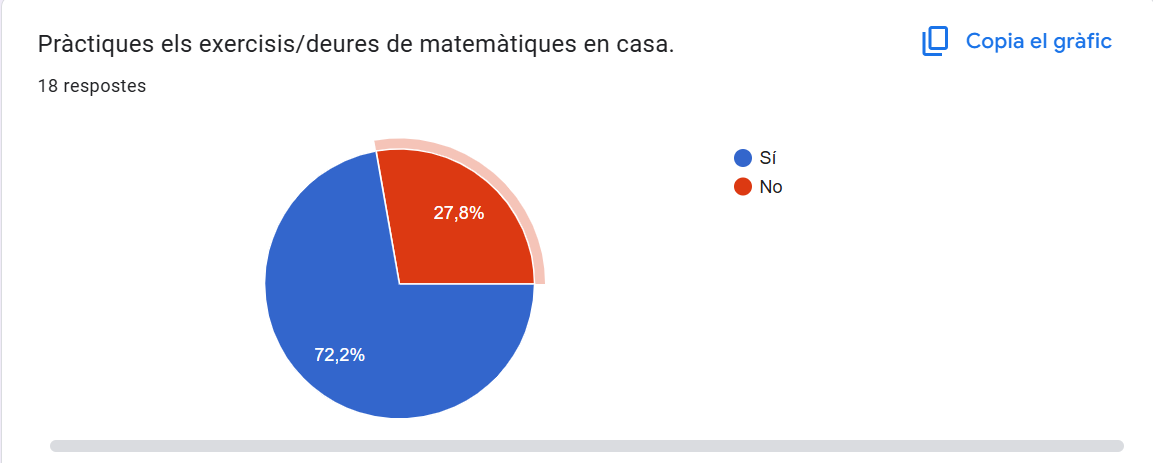
\includegraphics[width=0.5\textwidth]{./figures/19.png}
    \caption{Pràctiques a casa}
\end{figure}

\begin{figure}[H]
    \centering
    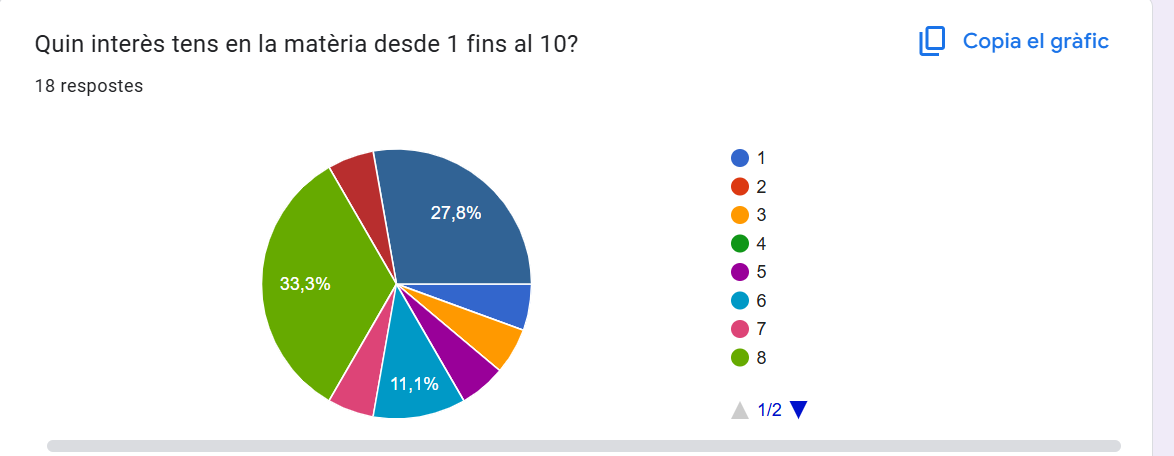
\includegraphics[width=0.5\textwidth]{./figures/20.png}
    \caption{Interès cap a l'assignatura}
\end{figure}
\end{comment}

\section{Xarxa neuronal de regressió}\label{sec:op}
Una intel·ligència artificial és un camp molt extens i, dins d’aquest, les xarxes neuronals també representen una branca àmplia i complexa. \\
En el nostre context utilitzarem un tipus concret de xarxa neuronal per a la pràctica: les \textbf{xarxes neuronals de regressió}.\\

Una xarxa neuronal de regressió, a diferència d’una de classificació, té una sortida de tipus lineal que permet predir un valor numèric continu. Aquest tipus de xarxes requereixen un conjunt de dades prou extens i ben estructurat per poder aprendre les relacions entre les variables d’entrada i generar una estimació fiable.\\

A continuació es mostra un esquema representatiu d’una xarxa neuronal de regressió:

\begin{center}[h!]
\centering
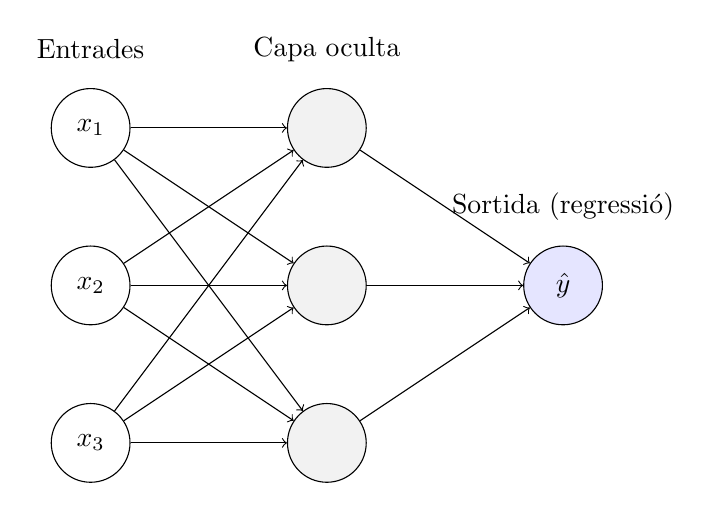
\begin{tikzpicture}[scale=1, transform shape]

% Input layer
\node[circle, draw, minimum size=1cm] (I1) at (0,2) {$x_1$};
\node[circle, draw, minimum size=1cm] (I2) at (0,0) {$x_2$};
\node[circle, draw, minimum size=1cm] (I3) at (0,-2) {$x_3$};

% Hidden layer
\node[circle, draw, fill=gray!10, minimum size=1cm] (H1) at (3,2) {};
\node[circle, draw, fill=gray!10, minimum size=1cm] (H2) at (3,0) {};
\node[circle, draw, fill=gray!10, minimum size=1cm] (H3) at (3,-2) {};

% Output layer
\node[circle, draw, fill=blue!10, minimum size=1cm] (O1) at (6,0) {$\hat{y}$};

% Connections input -> hidden
\foreach \i in {1,2,3}
  \foreach \h in {1,2,3}
    \draw[->] (I\i) -- (H\h);

% Connections hidden -> output
\foreach \h in {1,2,3}
  \draw[->] (H\h) -- (O1);

% Labels
\node at (0,3) {Entrades};
\node at (3,3) {Capa oculta};
\node at (6,1) {Sortida (regressió)};

\end{tikzpicture}
\small{Esquema d’una xarxa neuronal de regressió}
\end{center}

\section{Xarxa Neuronal amb llenguatge de programació}\label{sec:10}
En aquest apartat explicarem pas a pas de com vaig crear el nostre xarxa neuronal de regressió amb un llenguatge de programació.

\subsection{De celcius a fahrenheit}

Abans de començar a treballar amb la xarxa neuronal definitiu, vaig voler fer una de més simple per tal de coneixer amb més profunditat de com funciona una xarxa neuronal de regressió; en aquest cas he escollit un transformador d'unitats de temperatura, de celcius (\textbf{Unitat de temperatura basada en el punt de fusió de l'aigua}) a fahrenheit (\textbf{Sistema d'unitat basada en el punt d'ebullició i solidificació de l'aigua}). Per crear aquesta xarxa vaig escollir el Python com a llenguatge de programació, i el motiu esta explicat en l'apartat \ref{sec:4.4}.\\


Per començar, importo el framework i la biblioteca de Python que són les bases de dades necessàries per a la creació de la xarxa neuronal: \texttt{TensorFlow} (\textbf{framework}) i \texttt{{numpy}} (\textbf{biblioteca}). Com podeu veure, he creat uns \textit{abrevacions} per a poder-los cridar més fàcilment quan els necessiti.

\begin{itemize}
 \item \textbf{TensorFlow: }\label{TensorFlow} TensorFlow és un tipus de framework en que ofereix eines per crear i entrenar models de Ml (Machine learning) i Dl (Deep learning), biblioteques per programar xarxes neuronals i altres algoritmes, Compatibilitat amb GPU i TPU per accelerar càlculs, TensorBoard per visualitzar i monitorar entrenaments, Models preentrenats i repositoris, APIs (Application Programming Interface) en diversos llenguatges.
 \item \textbf{numpy: }\label{numpy} numpy és una biblioteca científica per treballar amb vectors i matrius.
\end{itemize}
\begin{figure}[H]
    \centering
    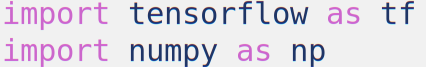
\includegraphics[width=0.5\textwidth]{./figures/1.png}
    \caption{Framework i biblioteca del Python}
\end{figure}


Agafo les paraules \textbf{celsius} i \textbf{fahrenheit} i les defineixo com a variables amb un signe \texttt{=}. Després poso \texttt{np} per indicar la biblioteca, seguit de \texttt{.array()} per especificar que és una llista. Dins dels parèntesis hi poso \texttt{[ ]} i a dins, els diferents valors de temperatura. Finalment, afegeixo el paràmetre \texttt{dtype=float} per indicar que es tracta de dades numèriques decimals.\\

Repeteixo el mateix procés amb \textbf{fahrenheit}, però en aquest cas les dades no poden ser arbitràries, sinó que han de ser les temperatures corresponents a les de \textbf{celsius} convertides a Fahrenheit. D’aquesta manera, la xarxa neuronal pot entendre la relació entre les dues sèries de dades.


\begin{figure}[H]
    \centering
    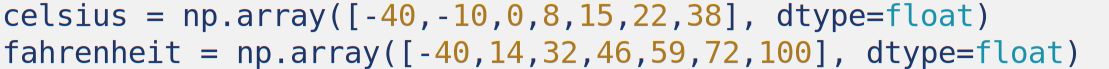
\includegraphics[width=0.5\textwidth]{./figures/2.png}
    \caption{Agrupació de dades amb numpy}
\end{figure}

Per començar, defineixo les capes de la xarxa neuronal. Utilitzant \texttt{tf.keras.layers.Dense} (\textbf{funció per a capes denses} (Keras és un tipus de API)), creo la primera capa oculta amb el paràmetre \texttt{units=3} per especificar que tingui \textbf{3 neurones}, i \texttt{input\_shape=[1]} per indicar que l'entrada és un sol valor. Li assigno el nom \texttt{oculte\_1}.\\
Repeteixo el procés per a la segona capa oculta, \texttt{oculte\_2}, amb \texttt{units=3} neurones també, però sense especificar \texttt{input\_shape} ja que la xarxa ho dedueix automàticament de la capa anterior.\\
Finalment, defineixo la capa de \texttt{sortida} amb \texttt{units=1} perquè retorni un sol valor (la predicció en Fahrenheit).\\
Amb totes les capes creades, les integro en un model seqüencial amb \texttt{tf.keras.Sequential}, passant-les dins d'una llista \texttt{[ ]} en l'ordre correcte: \texttt{[oculte\_1, oculte\_2, sortida]}. Això crea l'estructura bàsica de la nostra xarxa neuronal.


\begin{figure}[H]
    \centering
    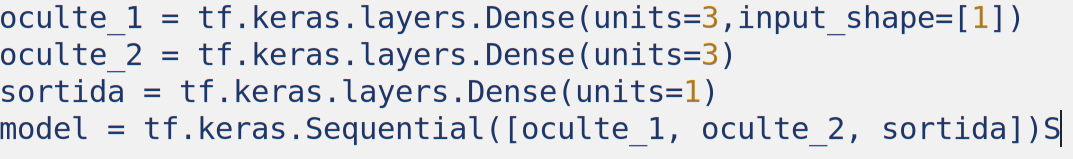
\includegraphics[width=0.5\textwidth]{./figures/3.png}
    \caption{Capes ocultes i la sortida d'una xarxa neuronal}
\end{figure}


Després de dissenyar l’estructura de la xarxa neuronal, cal ensenyar al model com aprendre i entrenar-se.
Per fer-ho utilitzem la variable \textbf{model}, a la qual ja havíem assignat les capes ocultes i la capa de sortida.
Tot seguit afegim la instrucció \textbf{.compile()}, que serveix per configurar el model abans de començar l’entrenament.

Dins de \texttt{.compile()} especifiquem el paràmetre \textbf{optimizer}, que indica la manera com el model ajustarà els pesos.
En aquest cas utilitzem \texttt{"adam"}, un optimitzador adaptatiu que redueix la velocitat d’aprenentatge quan detecta canvis bruscos en un pes,
l’augmenta quan el pes és estable i, alhora, recorda la direcció correcta per evitar oscil·lacions innecessàries.

A continuació, definim la funció de pèrdua amb el paràmetre \textbf{loss=\texttt{"mean\_squared\_error"}}.
La funció de pèrdua (\textit{loss}) mesura l’error del model i guia el procés d’aprenentatge.
En aquest cas, l’opció \texttt{mean squared error} (MSE, error quadràtic mitjà) és especialment útil en problemes de regressió,
ja que penalitza més fortament els errors grans i permet aconseguir prediccions més precises.


\begin{figure}[H]
    \centering
    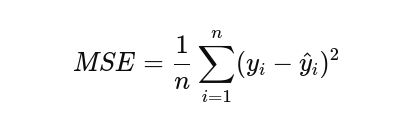
\includegraphics[width=0.5\textwidth]{./figures/5.png}
    \caption{Funció de pèrdua}
\end{figure}


\begin{figure}[H]
    \centering
    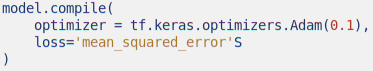
\includegraphics[width=0.5\textwidth]{./figures/4.png}
    \caption{Optimizació de la xarxa neuronal}
\end{figure}

Ara cal incloure la part crucial d'una xarxa neuronal: l'entrenament. Per fer-ho, utilitzem la variable \texttt{historial} per guardar l'evolució de l'entrenament i el model definit, \texttt{model}, aplicant-li el mètode \texttt{.fit()} que es el atribut que indica entrenament. Dins \texttt{.fit()} especifiquem, en ordre, les dades d'entrada (\texttt{celcius}), les dades de sortida (\texttt{fahrenheit}), el nombre de vegades que s'entrenarà la xarxa (\texttt{epochs=100}) i si volem mostrar el procés per pantalla (\texttt{verbose=1}, on 1 significa que sí i 0 que no).

A més, podem utilitzar \texttt{print()} per escriure comentaris o textos al terminal; en aquest cas hem posat \texttt{"Començem a entrenar..."} abans de començar i \texttt{"Model entrenat!"} un cop finalitzat l'entrenament.

\begin{figure}[H]
    \centering
    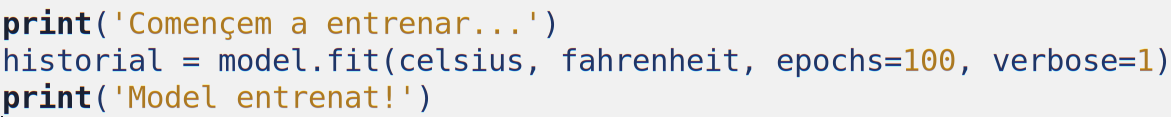
\includegraphics[width=0.5\textwidth]{./figures/6.png}
    \caption{L'entrenament de la xarxa neuronal}
\end{figure}
\label{matplotlib}
Després d’haver entrenat la xarxa neuronal i emmagatzemat l’evolució de la pèrdua a la variable \texttt{historial}, podem visualitzar com ha canviat la pèrdua a cada època utilitzant \texttt{matplotlib.pyplot}, una biblioteca de Python per crear gràfiques.\\

Primer, importem la biblioteca amb \texttt{import matplotlib.pyplot as plt}. A continuació, etiquetem els eixos de la gràfica amb \texttt{plt.xlabel("\# Època")} i \texttt{plt.ylabel("Magnitud de pèrdua")} per indicar què representa cada eix.\\

Per dibuixar la corba de la pèrdua utilitzem \texttt{plt.plot(historial.history[``loss''])}, que accedeix a la llista de valors de pèrdua que Keras ha guardat per cada època durant l’entrenament. Finalment, amb \texttt{plt.show()} mostrem la gràfica en una finestra del terminal o del notebook.\\

D’aquesta manera podem observar visualment si el model aprèn correctament, com disminueix la pèrdua al llarg de les èpoques i si hi ha comportaments irregulars que requeririen ajustar els paràmetres d’entrenament.

\begin{figure}[H]
    \centering
    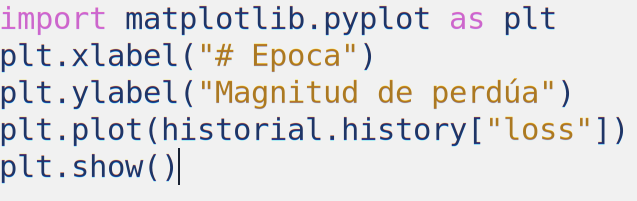
\includegraphics[width=0.5\textwidth]{./figures/7.png}
    \caption{La corba de pèrdua}
\end{figure}

Després d’haver entrenat la xarxa neuronal, podem fer prediccions amb nous valors d’entrada. Primer, utilitzem \texttt{print("Fem una predicció!")} per mostrar un missatge al terminal indicant que comença la predicció.\\

A continuació, fem servir \texttt{model.predict()} per calcular la predicció de la xarxa neuronal. En aquest cas, introduïm un valor de 100 graus Celsius amb \texttt{np.array([[100.0]], dtype=float)}, assegurant-nos que sigui un valor numèric decimal. El resultat s’emmagatzema a la variable \texttt{resultat}.\\

Finalment, utilitzem \texttt{print("El resultat es " + str(resultat) + " fahrenheit")} per mostrar la predicció obtinguda en Fahrenheit(el str es perque el variable resultat no sigui numeric sino un text). D’aquesta manera podem veure com el model converteix qualsevol temperatura de Celsius a Fahrenheit després de l’entrenament.


\begin{figure}[H]
    \centering
    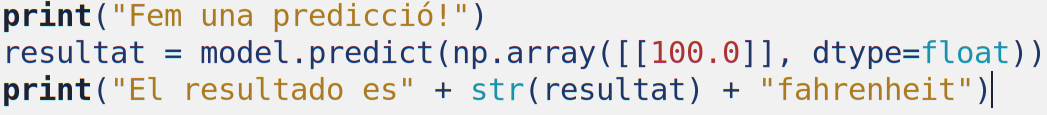
\includegraphics[width=0.5\textwidth]{./figures/8.png}
    \caption{Resultat de la predicció}
\end{figure}

Per a inspeccionar els pesos interns de la xarxa neuronal, podem utilitzar el mètode \texttt{.get\_weights()} en cada capa. Si el posem en els variables que haviem assignat les capes, per exemple, \texttt{oculte\_1.get\_weights()}, \texttt{oculte\_2.get\_weights()} i \texttt{sortida.get\_weights()} permeten veure els valors dels pesos i els biaixos que el model ha après durant l’entrenament, mostrant-los amb \texttt{print()}.


\begin{figure}[H]
    \centering
    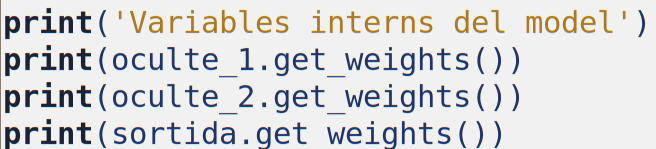
\includegraphics[width=0.5\textwidth]{./figures/9.png}
    \caption{Els pesos i biaixos assignats}
\end{figure}

Aquí hi és una mostra del resultat que dona:

\begin{figure}[H]
    \centering
    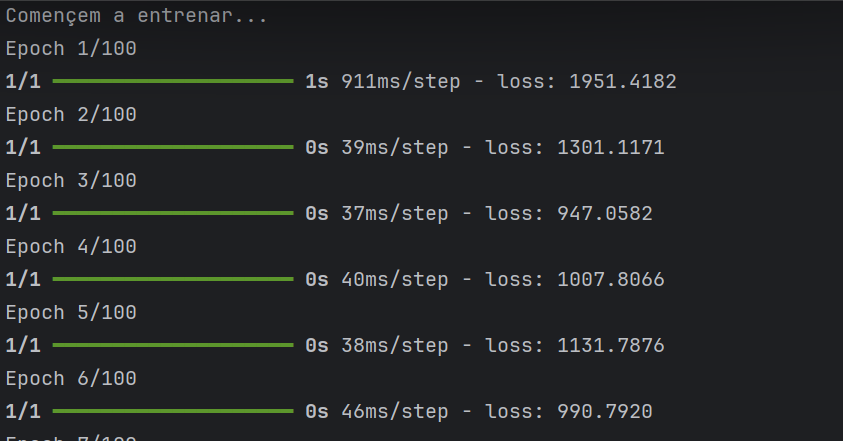
\includegraphics[width=0.5\textwidth]{./figures/10.png}
    \caption{El inicí de l'entrenament de la xarxa neuronal}
\end{figure}

\begin{figure}[H]
    \centering
    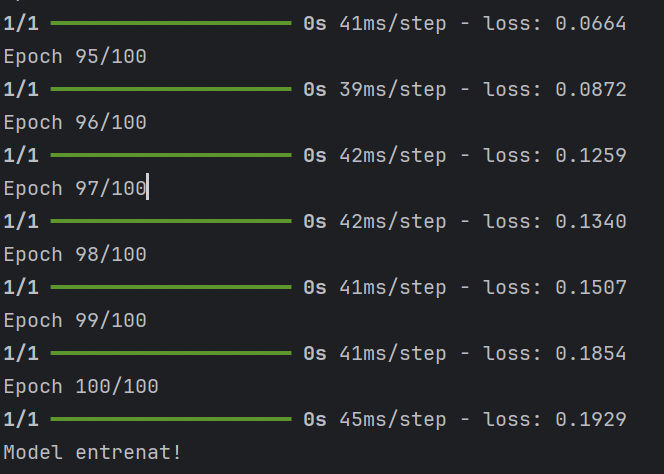
\includegraphics[width=0.5\textwidth]{./figures/11.png}
    \caption{Model entrenat}
\end{figure}


\begin{figure}[H]
    \centering
    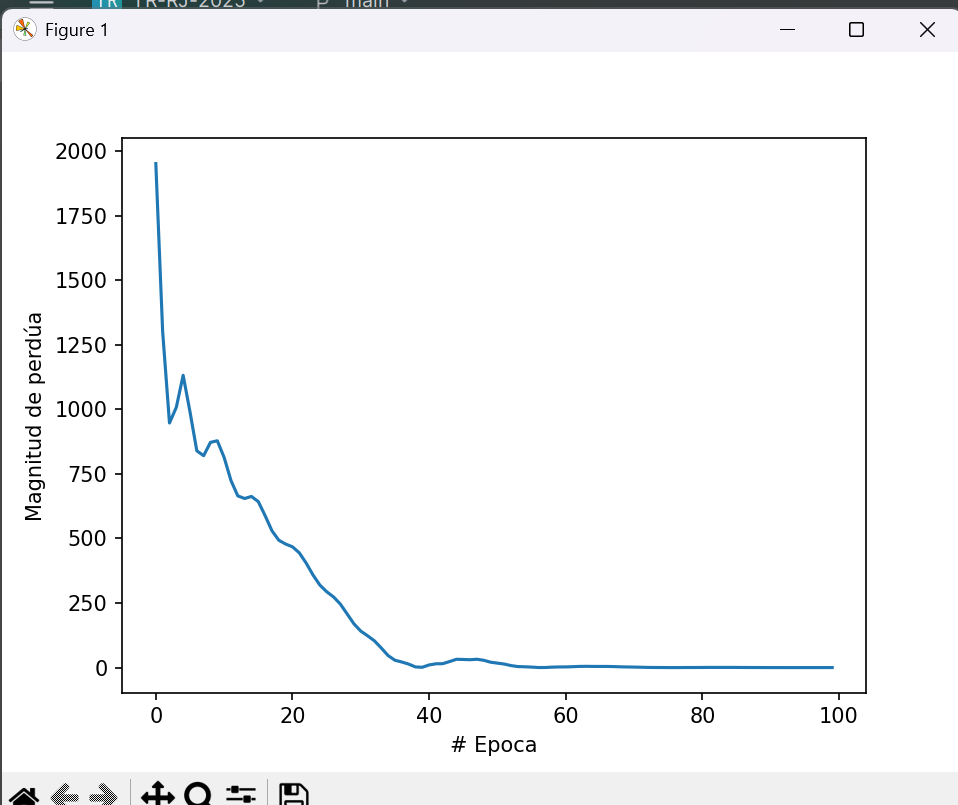
\includegraphics[width=0.5\textwidth]{./figures/12.png}
    \caption{Gràfica de la corba de pèrdua}
\end{figure}


\begin{figure}[H]
    \centering
    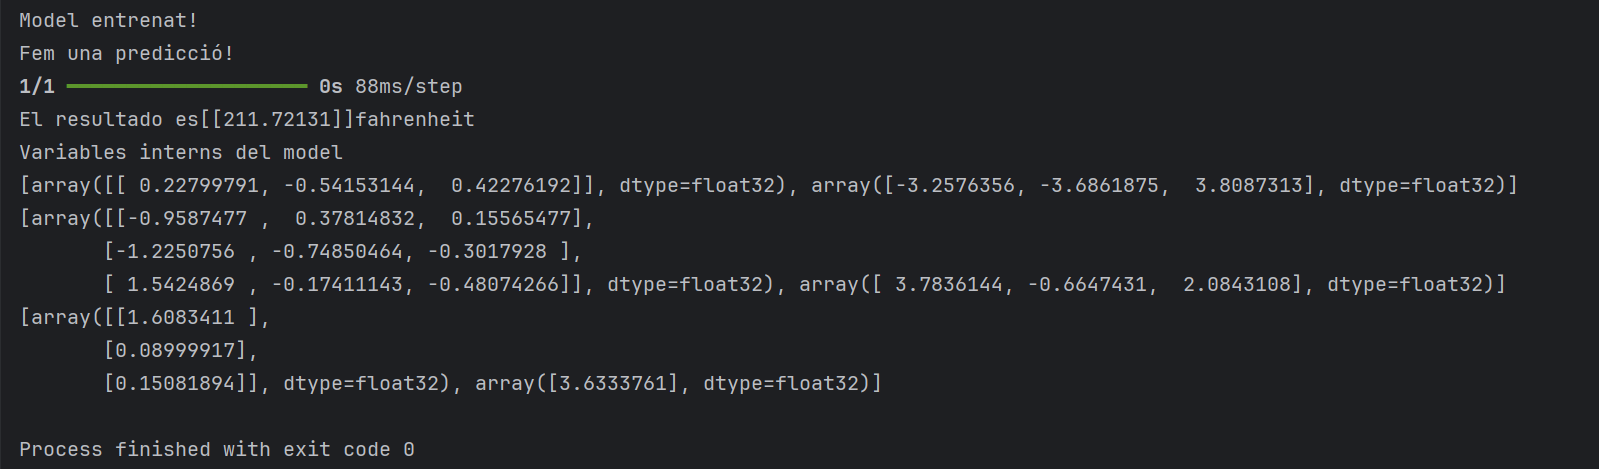
\includegraphics[width=0.5\textwidth]{./figures/13.png}
    \caption{El resultat de la predicció suposant que són 100 celcius el que ha de transformar i els baixos i pesos que ha utilizat la xarxa neuronal}
\end{figure}


Font: (\href{https://www.youtube.com/watch?v=iX_on3VxZzkhttps://www.youtube.com/watch?v=iX_on3VxZzk}{Xarxa neuronal amb Python})

\subsection{Predicció de les notes finals de matematiques }
Una vegada treballat amb la xarxa neuronal de celcius a fahrenheit, ja em trobo capacitat per fer la xarxa neuronal que ens haviem proposat, explicat en l'apartat \ref{sec:intr}

Igual que la xarxa neuronal de celcius a fahrenheit, començare amb la importació dels framework i biblioteques necessaries pel treball: \texttt{numpy}, \texttt{TensorFlow}, \texttt{matplotlib}, \texttt{MinMaxScaler}, \texttt{random} i \texttt{os}

\begin{itemize}
 \item \textbf{MinMaxScaler: } MinMaxScaler és una eina de la llibreria sklearn, la seva funció es normalitzar les dades i convertir els valors numerics dins del rang $[0,1]$, en que facilitarà molt la feina de la xarxa neuronal en entendre les relacions numerics. \nameref{subsec:24}
 \item \textbf{random: } random és una llibreria bàsica del Python, aquest modul genera i selecciona nombres aleatoris.
 \item \textbf{os: } os també és una llibreria estandard del Python. el que ofereix aquest modul és per treballar amb el sistema operatiu.
\end{itemize}

\begin{figure}[H]
    \centering
    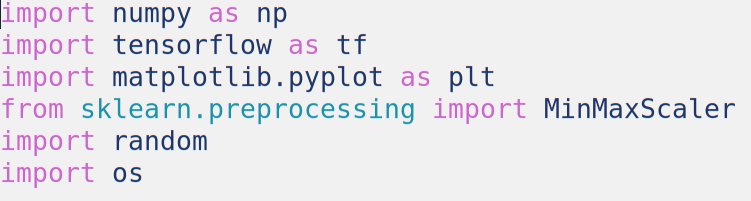
\includegraphics[width=0.5\textwidth]{./figures/21.png}
    \caption{Els biblioteques, llibreries i framework}
\end{figure}

A diferència de l’anterior xarxa, aquesta vegada he de fixar els resultats de la predicció per tal que les notes finals siguin més precises. Amb l’ajuda de la llibreria random pugues seleccionar qualsevol nombre aleatori que vulguessí, però per garantir la reproduïbilitat assignem la llavor (seed) amb el valor 42. Així, la xarxa neuronal sempre s’inicialitzarà amb els mateixos pesos i biaixos.\\

A continuació, controlo l’aleatorietat de les diferents llibreries que intervenen en el procés: \texttt{NumPy}, \texttt{TensorFlow}, \texttt{random} i, finalment, estableixo el valor del hash de Python amb la importació del mòdul \texttt{os}.

Control de l’aleatorietat:
\begin{itemize}
\item \textbf{Llavor:} \texttt{seed = 42}
\item \textbf{NumPy:} \texttt{np.random.seed(seed)}
\item \textbf{TensorFlow:} \texttt{tf.random.set\_seed(seed)}
\item \textbf{random:} \texttt{random.seed(seed)}
\item \textbf{Python:} \texttt{os.environ["PYTHONHASHSEED"] = str(seed)}
\end{itemize}

\begin{figure}[H]
    \centering
    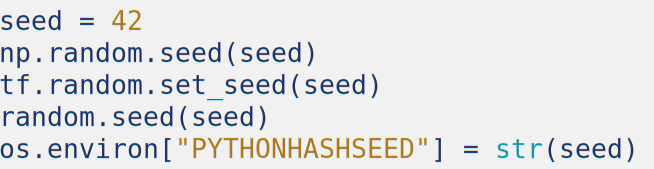
\includegraphics[width=0.5\textwidth]{./figures/22.png}
    \caption{Fixar els resultats de les prediccions}
\end{figure}


Una vegada fixats els pesos i els biaixos, començo a emmagatzemar les dades per a l’entrenament de la xarxa neuronal.
Primer preparo les dades d’entrada, que anomenaré \texttt{X}, seguint aquest ordre de variables:

\begin{enumerate}
    \item Realització de deures
    \item Hores d’estudi setmanals
    \item Hores de secció
    \item Interès en la matèria
    \item Nota del segon trimestre
    \item Nota del tercer trimestre
\end{enumerate}

Definim \texttt{X = np.array([])}, que crea una llista de dades.
D’aquesta manera, només caldrà anar omplint-la amb les dades obtingudes del formulari, mantenint sempre l’estructura
\texttt{[x1, x2, x3, x4, x5, x6]}.
Finalment, afegeixo \texttt{dtype=float} per indicar que els valors són decimals.

Un cop assignades les dades d’entrada, toca construir les dades de sortida, també anomenades resultat o valor, que representaré amb \texttt{y}.
A diferència de \texttt{X}, la sortida \texttt{y} només tindrà una columna, que correspondrà al valor que genera cada fila i columna de \texttt{X}, separada per comes.

\begin{figure}[H]
    \centering
    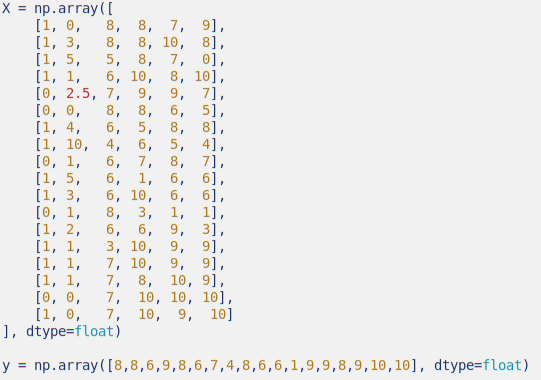
\includegraphics[width=0.5\textwidth]{./figures/23.png}
    \caption{magatzem de dades}
\end{figure}

A més d’emmagatzemar les dades, m’he adonat que la normalització també és crucial perquè la xarxa neuronal pugui entendre millor les relacions entre les dades. Això és degut al fet que cada dada pot tenir un valor numèric molt diferent, com les hores d’estudi o si s’ha estudiat o no. Per normalitzar les dades utilitzarem el \texttt{MinMaxScaler} de \texttt{sklearn}, tant per a la \texttt{X} com per a la \texttt{y}.\\

Primer, creem un escalador per a la \texttt{X} amb \texttt{scaler = MinMaxScaler()}. A continuació, apliquem la normalització amb \texttt{X\_scaled = scaler.fit\_transform(X)}, amb la qual cosa totes les dades de la \texttt{X} quedaran dins l’interval $[0,1]$.\\

De manera similar, normalitzarem la \texttt{y} amb un altre escalador, \texttt{scaler\_y}. Aquí cal convertir \texttt{y} en una matriu amb \texttt{y.reshape(-1, 1)} ja que el \texttt{MinMaxScaler} només funciona amb matrius de dues dimensions. Després, apliquem la normalització amb \texttt{y\_scaled = scaler\_y.fit\_transform(y.reshape(-1, 1))}.


\begin{figure}[H]
    \centering
    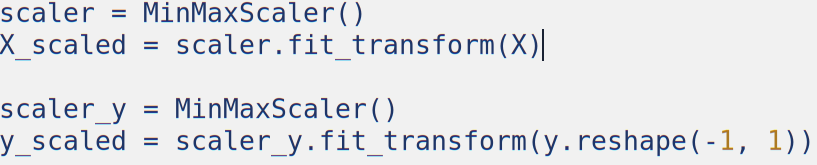
\includegraphics[width=0.5\textwidth]{./figures/24.png}
    \caption{Normalització de les dades}
\end{figure}

\begin{figure}[H]
    \centering
    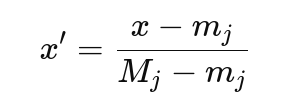
\includegraphics[width=0.5\textwidth]{./figures/25.png}
    \caption{Normalització Min-Max}
\end{figure}


Un cop normalitzades les dades, el següent pas és definir l’estructura de la xarxa neuronal que utilitzare per predir les notes finals de matemàtiques. Per a això, he creat un model seqüencial amb capes ocultes.

\begin{itemize}
    \item \textbf{Primera capa oculta:} \texttt{tf.keras.layers.Dense(32, activation="relu", input\_shape=[6])} \\
    Aquesta capa té \textbf{32 neurones} i utilitza la funció d’activació \texttt{ReLU} (\textit{Rectified Linear Unit}) per introduir no-linealitat. El paràmetre \texttt{input\_shape=[6]} indica que cada mostra d’entrada té 6 característiques, corresponents a les variables definides a \texttt{X}.

    \item \textbf{Segona capa oculta:} \texttt{tf.keras.layers.Dense(16, activation="relu")} \\
    Aquesta capa té \textbf{16 neurones} i també utilitza \texttt{ReLU}. No cal especificar \texttt{input\_shape} ja que el model dedueix automàticament l’entrada de la capa anterior.

    \item \textbf{Capa de sortida:} \texttt{tf.keras.layers.Dense(1)} \\
    La capa final té \textbf{una sola neurona}, ja que vull obtenir un sol valor com a predicció: la nota final. No he posat una funció d'activació perquè la funcio que doni sigui lineal.
\end{itemize}

\begin{figure}[H]
    \centering
    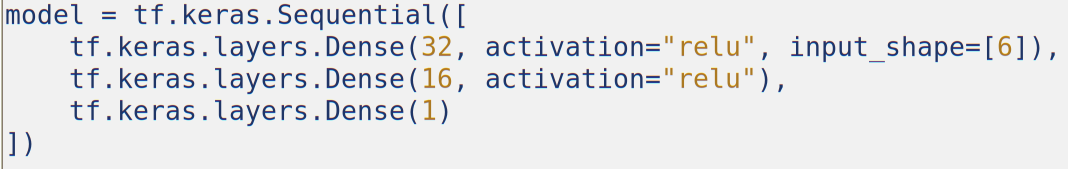
\includegraphics[width=0.5\textwidth]{./figures/26.png}
    \caption{Estructura de la xarxa neuronal}
\end{figure}

Després de definir l’estructura de la xarxa neuronal, cal configurar com el model aprendrà. Per fer-ho, utilitzem el mètode \texttt{.compile()} del model, que permet establir l’optimitzador, la funció de pèrdua i les mètriques d’avaluació.

\begin{itemize}
    \item \textbf{Optimitzador:} \texttt{tf.keras.optimizers.Adam(0.01)} \\
    L’optimitzador \texttt{Adam} és un algoritme adaptatiu que ajusta automàticament la velocitat d’aprenentatge dels pesos. El paràmetre \texttt{0.01} indica la taxa d’aprenentatge inicial. Aquest optimitzador és especialment eficient per a problemes de regressió i xarxes amb múltiples capes.

    \item \textbf{Funció de pèrdua:} \texttt{"mean\_squared\_error"} \\
    La funció de pèrdua (\textit{loss}) mesura l’error del model durant l’entrenament. En aquest cas, \texttt{mean squared error (MSE)} penalitza més fortament els errors grans, ajudant la xarxa a generar prediccions més precises.

    \item \textbf{Mètrica:} \texttt{["mae"]} \\
    La mètrica \texttt{Mean Absolute Error (MAE)} permet monitorar l’error absolut mitjà entre les prediccions i els valors reals, facilitant la interpretació del rendiment del model durant l’entrenament.
\end{itemize}

\begin{figure}[H]
    \centering
    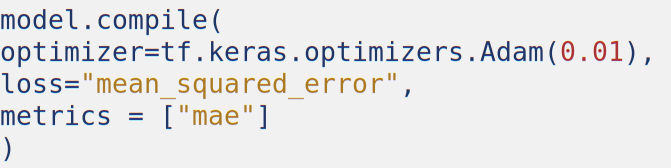
\includegraphics[width=0.5\textwidth]{./figures/27.png}
    \caption{Configuració de la xarxa}
\end{figure}

Un cop compilat el model, el següent pas és ensenyar-lo a aprendre de les dades. Per això utilitzem el mètode \texttt{.fit()}, que ajusta els pesos de la xarxa neuronal per minimitzar l’error de predicció. En aquest cas, utilitzare les dades normalitzades \texttt{X\_scaled} i \texttt{y\_scaled}, de manera que l’aprenentatge sigui estable i eficient. El model s’entrena durant 400 èpoques, és a dir, passarà 400 vegades per totes les mostres d’entrenament ajustant els pesos en cada iteració. A més, s’ha activat l’opció \texttt{verbose=1} per mostrar per pantalla el progrés de l’entrenament i l’error de cada època.

Per visualitzar l’evolució de la pèrdua al llarg de l’entrenament, utilitzare \texttt{matplotlib.pyplot}. La funció \texttt{plt.plot(historial.history["loss"])} dibuixa la corba de la pèrdua (\textit{loss}) per cada època. Els eixos de la gràfica s’etiqueten amb \texttt{plt.xlabel("Època")} i \texttt{plt.ylabel("Pèrdua (loss)")}, i finalment \texttt{plt.show()} mostra la gràfica amb la corba de pèrdua.

\begin{figure}[H]
    \centering
    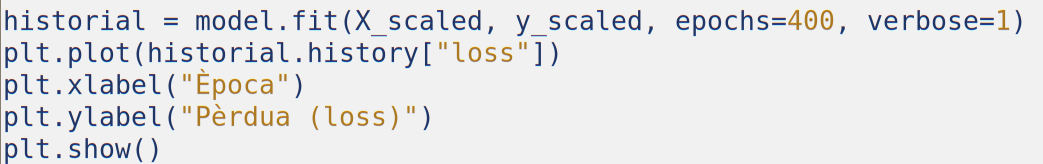
\includegraphics[width=0.5\textwidth]{./figures/28.png}
    \caption{Entrenament de la xarxa i la corba de pèrdua}
\end{figure}

Ara que la xarxa neuronal ja està entrenada, vull mostrar els resultats. Primer, configuro una nova entrada amb les dades de la mostra que vull predir \texttt{nou\_entrada = np.array([[1, 0,   7,  10,  9,  10]])} i la normalitzo amb el mateix escalador que vaig utilitzar durant l’entrenament \texttt{nou\_entrada\_scaled = scaler.transform(nou\_entrada)}, per assegurar-me que els valors es troben dins del mateix rang. Un cop normalitzada, demano a la xarxa neuronal que realitzi la predicció \texttt{prediccio = model.predict(nou\_entrada\_scaled)}. Com que la sortida original estava escalada i convertida en una matriu, inverteixo aquesta transformació per obtenir la predicció en l’escala real \texttt{prediccio\_real = scaler\_y.inverse\_transform(prediccio)}. Finalment, mostro el resultat amb \texttt{print("Nota prevista:", round(prediccio\_real[0][0],2))}, arrodonint-lo a les xifres que vull per facilitar-ne la lectura, el \texttt{[0][0]} és per seleccionar la primera fila del matriu i el primer element d'aquesta fila, i el \texttt{round(,2)} es per arrodonint-lo en dos xifres. D’aquesta manera, finalitzo tot el procés de predicció amb la xarxa neuronal.


\begin{figure}[H]
    \centering
    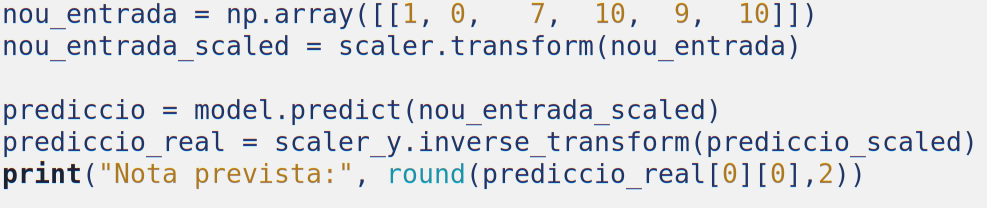
\includegraphics[width=0.5\textwidth]{./figures/29.png}
    \caption{Resultat final i els seus ajustaments}
\end{figure}




\section{Xarxa Neuronal amb fulls de calculs}\label{sec:11}
En aquest apartat continuarem amb la xarxa neuronal de regressió però aquesta vegada utilitzarem un full de càlculs per fer-ho.
L'estructura que utilitzarem per a aquesta pràctica serà la del perceptró.

\begin{figure}[H]
    \centering
    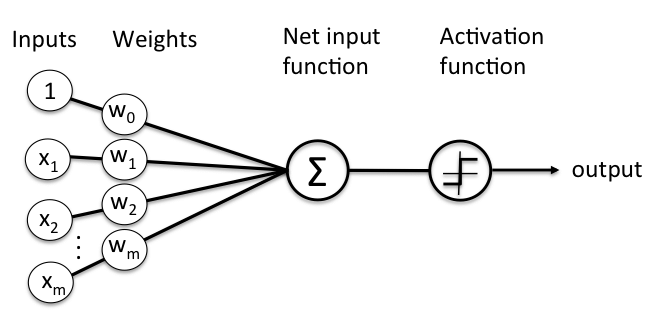
\includegraphics[width=0.5\textwidth]{./figures/perceptro.png}
    \caption{Estructura del perceptró}
\end{figure}

Ara començarem la pràctica ordenant les dades de cada alumne del formulari en el full de càlculs.

\begin{figure}[H]
    \centering
    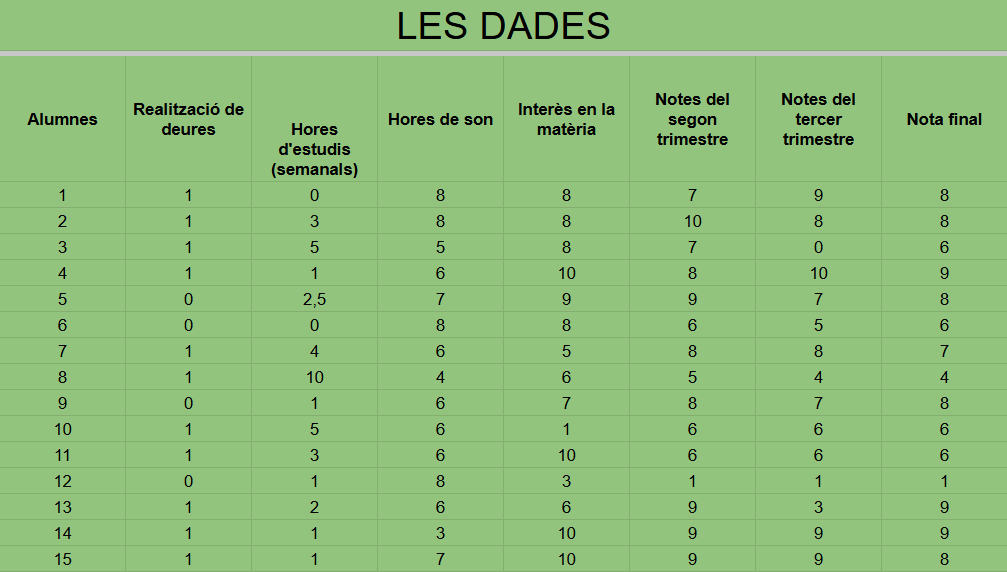
\includegraphics[width=0.5\textwidth]{./figures/Dades.png}
    \caption{Dades dels alumnes en el full de càlcul}
\end{figure}

Una vegada he ordenat tota la informació, he decidit representar els valors d'entrada d'una forma més senzilla d'entendre i curta, anomenant-los $xi$.
\begin{itemize}
 \item \textbf {Realització dels deures:} $x1$
 \item \textbf {Hores d'estudis:} $x2$
 \item \textbf {Hores de son:} $x3$
 \item \textbf {Interès en la matèria:} $x4$
 \item \textbf {Notes del segon trimestre:} $x5$
 \item \textbf {Notes del tercer trimestre:} $x6$
 \item \textbf {Nota final:}´ $y$
\end{itemize}

Aquesta representació queda així:

\begin{figure}[H]
    \centering
    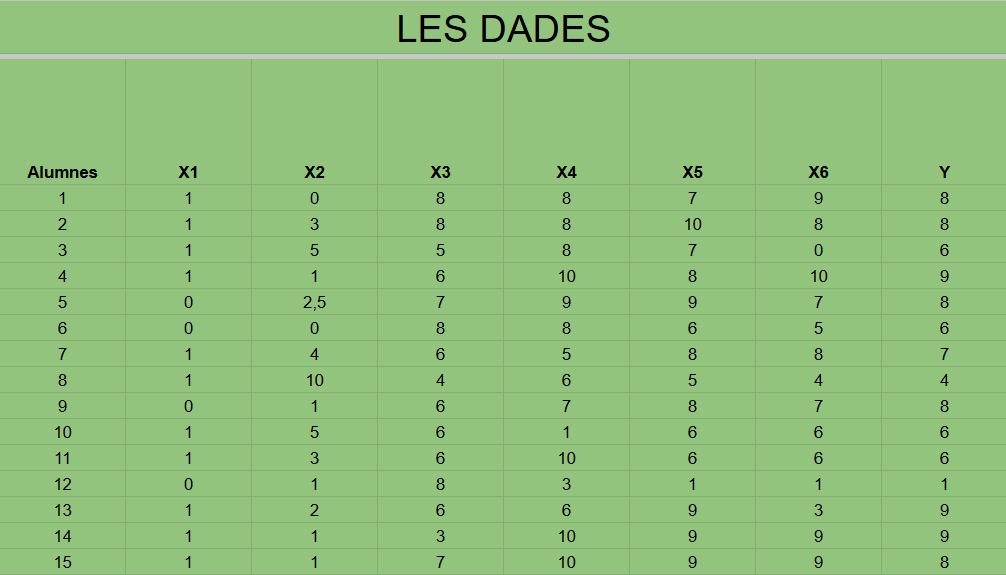
\includegraphics[width=0.5\textwidth]{./figures/Dades_resumides.png}
    \caption{Taula resumida}
\end{figure}

L'entrada de ``Realització de deures'' és una data binària que només pot prendre valors 0 o 1.
\subsection{Normalització de dades}\label{subsec:24}
Abans de continuar, és necessari explicar que és la normalització de dades.
La normalització de dades és una tècnica de processament que consisteix a transformar dades de diferents escales a una escala comuna, com per exemple del 0 a l'1, això facilita la comparació i l'anàlisi de la xarxa neuronal i millora el seu rendiment. En el nostre cas, tenim dades binàries i dades ordinàries que poden prendre qualsevol valor, aquest desequilibri afecta els càlculs posteriors si no se solucionen d'alguna manera. \\

Per aquesta raó, convertirem totes les dades en valors d'entre 0 i 1. Aquest procés implica calcular la mitjana de les dades i la desviació estàndard de cada variable. Per això utilitzant la fórmula següent:\\
$$z = \frac{x - \mu}{\sigma}$$\\

On:\\
$z$ És el valor normalitzat\\
$x$ És el valor original\\
$\mu$ És la mitjançan\\
$\sigma$ És la desviació estàndar\\

Aquests càlculs són fàcils d'obtenir amb les funcions que ens proporciona el full de càlcul.

\begin{figure}[H]
    \centering
    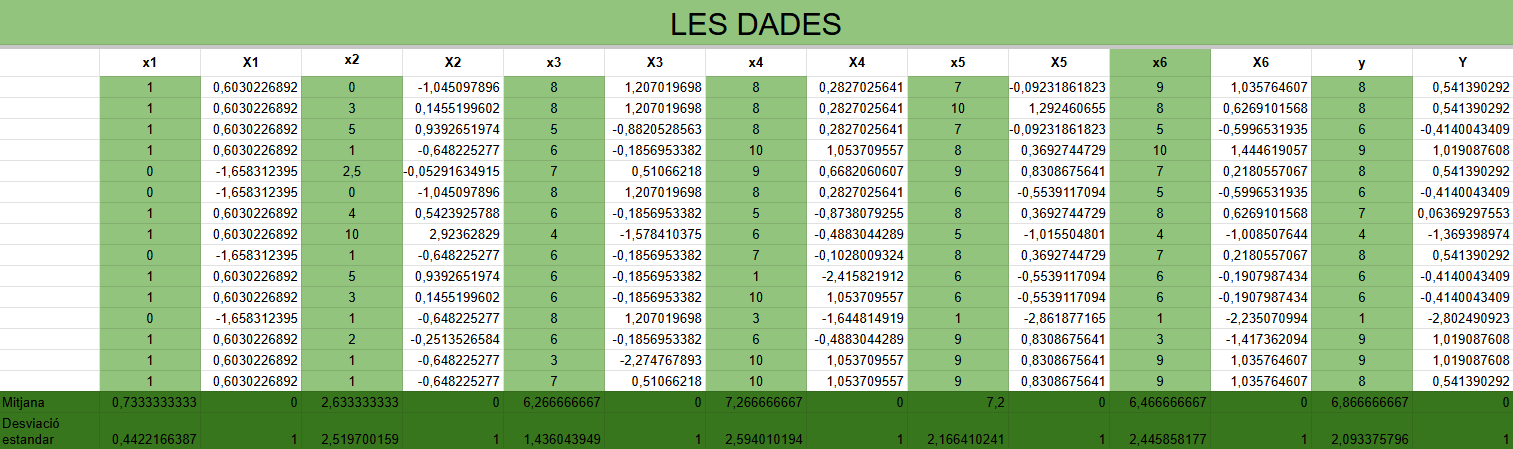
\includegraphics[width=0.5\textwidth]{./figures/Dades_normalitzades.png}
    \caption{Taula resumida}
\end{figure}

\subsection{Els paràmetres del model}
Ara que ja tenim totes les dades preparades, hem d'assignar a cada variable X el seu pes per determinar la seva importància en la predicció final. Al començament de l'entrenament, assignarem a tots els valors d'entrada el mateix pes, ja que es corregiran lentament durant l'entrenament.
També hem d'afegir el biaix, que és la constant que ajuda a millorar l'ajust de les prediccions.

\begin{figure}[H]
    \centering
    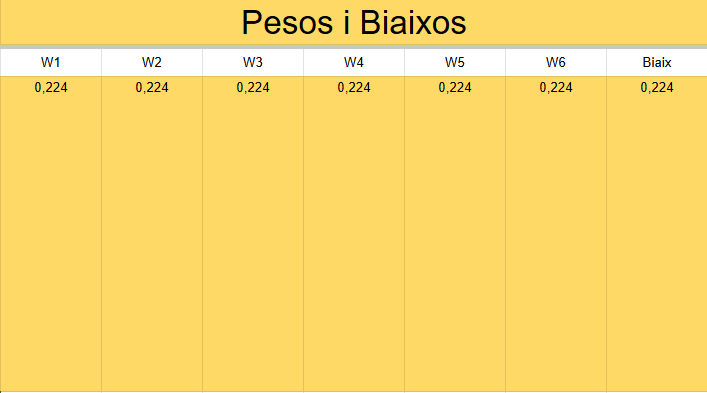
\includegraphics[width=0.5\textwidth]{./figures/Pesos.png}
    \caption{Taula dels pesos}
\end{figure}

En la figura 5.28, podem observar com ha quedat la taula després d'afegir els pesos als valors d'entrada, he afegit 6 columnes de pesos respecte a les 6 entrades i una columna més pel biaix.

\subsection{Funció d'error del model}
Fins ara, ja tenim les dades d'entrada normalitzades i els seus respectius pesos inicials assignats, ara podem aplicar la fórmula que s'utilitza en les xarxes neuronals per calcular la predicció temporal de la nota final. Hem de recordar que la fórmula és:\\
\[
\sum w_i x_i + \text{biaix}
\] \\
Després d'aplicar la fórmula, obtindrem la predicció de la nota final, tal com es veu en la figura 5.29.

\begin{figure}[H]
    \centering
    \includegraphics[width=0.5\textwidth]{./figures/Predicció.png}
    \caption{Prediccions del model}
 \end{figure}

Hem de recordar que els valors de la predicció són erronis, a que els pesos que hem assignat són aleatoris.

Per aquesta raó, el següent pas de la pràctica és entrenar el nostre model per millorar els paràmetres. Per dur això, haurem d'aplicar un procés d'optimització per ajustar aquests paràmetres. En aquest cas utilitzarem l'algoritme gradient descendent.

Començarem afegint més columnes en el nostre full en la nostra taula. Si restem els valors de la predicció ($Y$) amb els valors reals ($y$) obtindrem la diferència entre la nota dels alumnes i les notes predictives.

\begin{figure}[H]
    \centering
    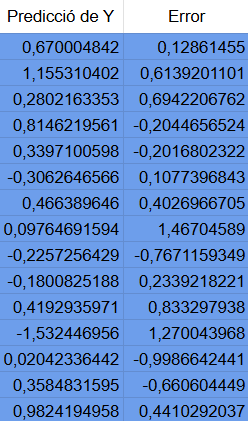
\includegraphics[width=0.5\textwidth]{./figures/Errors.png}
    \caption{Erros de la predicció}
\end{figure}

Es pot veure en la imatge 5.30 dues columnes addicionals, la columna ``error'' emmagatzema els errors del model i l'altre conté els mateixos errors, però en valor absolut, és a dir, que tots els valors estan en positiu, d'aquesta manera serà més fàcil apreciar la diferència dels errors en les prediccions i els càlculs dels paràmetres.\\

Després de crear aquestes taules, calcularem la mitjana dels valors que estan en la taula dels errors en positiu, el resultat d'aquesta mitjana ens ajudarà a orientar-nos i determinar si en cada iteració l'error està augmentant o disminuint, com més baix sigui aquest valor, la predicció serà més precisa.\\
\subsection{Canvis dels paràmetres}
Un cop tenim la funció d'error de la primera predicció, el pas següent és entrenar el model per ajustar els valors dels pesos i del biaix adequadament perquè les següents prediccions siguin més precises.
Per aconseguir això, hem de tindre en compte les dades següents: Quan la diferència de $Y$ respecte a $y$ és més gran, més lluny estaran els pesos dels seus valors ideals. Per tant, hem de trobar la forma de calcular de forma correcta els pesos respecte de la diferència dels valors de la predicció.

Gràcies a la fórmula de la xarxa neuronal sabem que si el valor d'entrada ($X$) és petit, el seu pes ($W$) també ho serà, ja que aquests es multipliquen. Hem de tindre en compte dues coses: La diferència de la predicció final ($Y$) i del valor real ($y$) i el valor d'entrada ($X$) respecte al seu pes ($W$). Per tant, fórmula que utilitzarem per calcular els canvis dels paràmetres serà:\\
$\Delta W = (Y_{\text{original}} - Y_{\text{predicció}}) \times X$\\
Aquesta fórmula serà la que ens ajudarà a ajustar els paràmetres per tal que la predicció sigui cada cop més precisa. Aplicant aquesta fórmula a cada una de les dades, obtindrem 7 columnes més.

\begin{figure}[H]
    \centering
    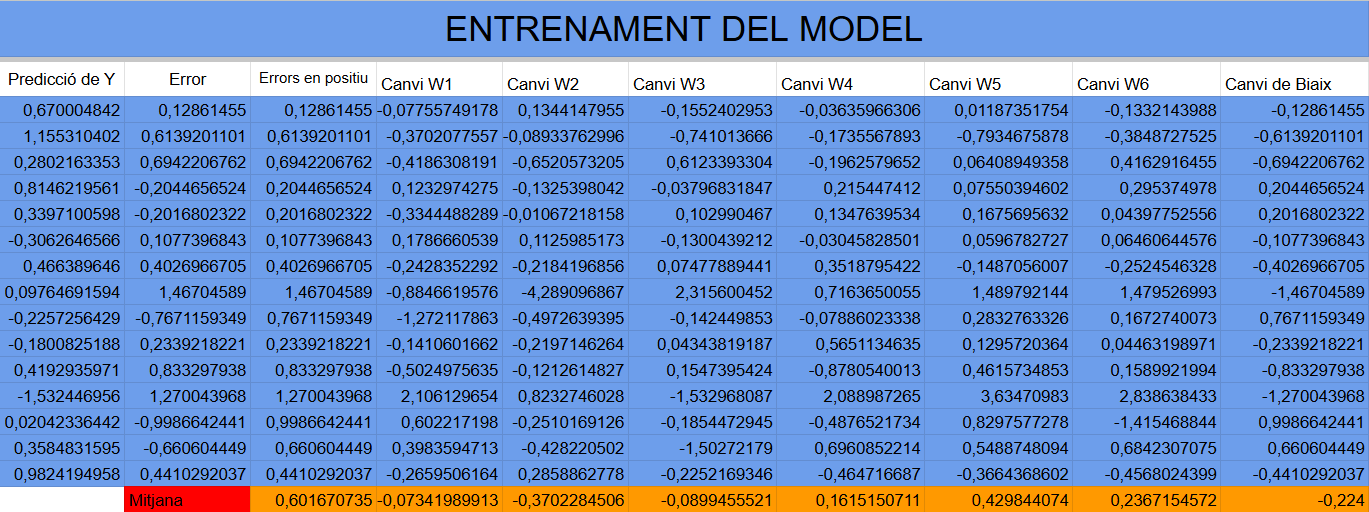
\includegraphics[width=0.5\textwidth]{./figures/Canvis.png}
    \caption{Canvis en els paràmetres}
\end{figure}

En la figura 5.31 es pot veure com han quedat aquestes taules, els canvis del biaix es calculen amb la mateixa fórmula que els pesos, però sense restar-li cap entrada, ja que actua com una entrada constant.\\

Ara és necessari calcular la mitjana dels canvis dels pesos, les mitjanes obtingudes a partir dels canvis seran uns dels valors que utilitzarem per ajustar els paràmetres.

\subsection{La taxa d'aprenentatge}
Abans de començar a entrenar el model, hem de parlar d'una variable molt important, que és la taxa d'aprenentatge. Aquesta taxa és un paràmetre que ajusta l'ample dels passos que fem per actualitzar els pesos i el biaix del model, el valor d'aquesta taxa no pot ser molt gran perquè si no no es podria trobar el punt de convergència, ni molt petit perquè ralentitzaria la xarxa.\\

Normalment, el valor de la taxa d'aprenentatge és 1, però de vegades aquest valor és molt gran i augmentaria l'error del model, si això passa hauríem de reduir el seu valor progressivament fins a un punt on l'error de la xarxa disminueixi significativament.\\
Finalment, per trobar el valor final dels canvis ajustats dels paràmetres haurem de multiplicar a mitjana dels canvis dels pesos per la taxa d'aprenentatge.
\subsection{Èpoques d'entrenament}
Ja podem començar a entrenar el model, ho farem copiant la mateixa taula que tenim a sota, com es veu en la figura 5.32.

\begin{figure}[H]
    \centering
    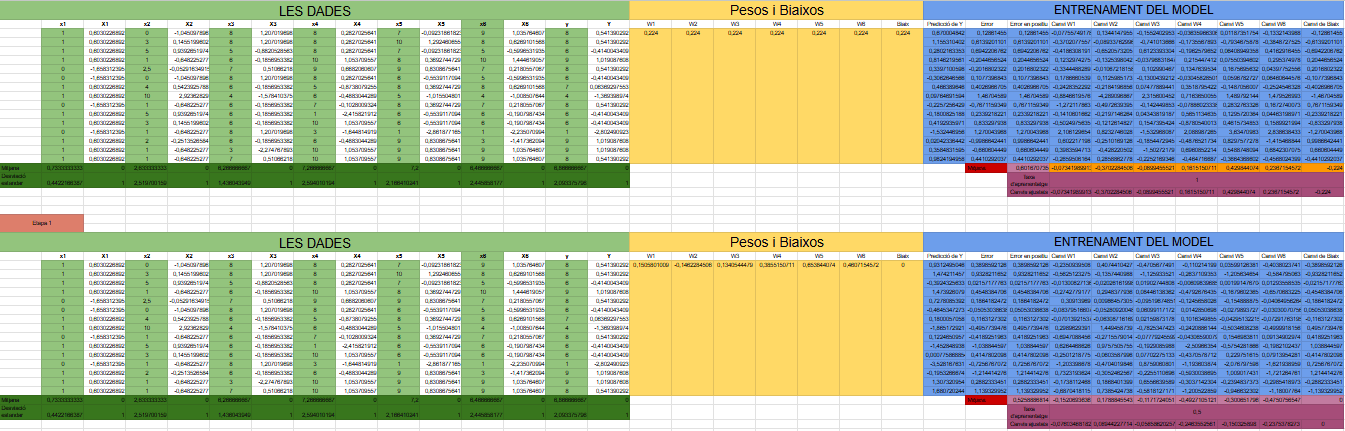
\includegraphics[width=0.5\textwidth]{./figures/Etapa_1.png}
    \caption{Èpoques d'entrenament}
\end{figure}

Cada època d'entrenament seria com si fos una iteració, podem veure que els paràmetres de la primera època han canviat respecte de la primera taula, que li anomenarem època 0, on aquests paràmetres eren inicialment aleatoris, el valor del primer pes de l'època 1 ($W1$) es calcula sumant el pes de l'època 0 pel valor del canvi ajustat.\\
Per saber si el model ha millorat, la millor forma de comprovar-ho és fixant-se en la taula dels errors en positiu. Podem veure que aquest valor ha disminuït respecte a l'època anterior, això significa que està millorant.\\
A partir d'ara hem de fer-ho mateix repetidament fins que el canvi de l'error entre les èpoques siguin molt petits, quan passi això significarà que estem pràcticament en el punt de convergència, i és important anant ajustant la taxa d'aprenentatge.
\subsection{Resultats}
En aquest cas, ha calgut 8 etapes per arribar al punt de convergència. He organitzat els valors de l'error de cada època en una gràfica perquè sigui més fàcil visualitzar els canvis.


\begin{figure}[H]
    \centering
    \includegraphics[width=0.5\textwidth]{./figures/Gràfica_error.png}
    \caption{Gràfica dels valors d'error en cada època}
\end{figure}


En la figura 5.33, podem apreciar que l'error ha disminuït dràsticament entre l'època 0 fins a l'època 4, però després de la cinquena època l'error pràcticament no s'ha mogut, vaig ajustar la taxa d'aprenentatge moltes vegades, però l'error encara baixava molt lentament, fins que vaig arribar a l'etapa 8. Això vol dir que el model no podia ajustar més els pesos.
